\documentclass{beamer}

\usepackage[utf8x]{inputenc}
\usepackage{default}
%Configurações gerais
\usetheme{PaloAlto}
\usecolortheme{seahorse}

\title{Sistemas Digitais 2\\ \textbf{Introdução a Máquina de Estados Finita}}
\author{Rodrigo Siqueira}
\date{\today}
\institute{\textbf{Universidade de Brasília - Faculdade do Gama}} 

\begin{document}

%SLIDE INICIAL DE APRESENTAÇÃO
\begin{frame}
  \titlepage
\end{frame}

%SLIDES == INTRODUÇÃO
\section{Introdução}
\begin{frame}
  \frametitle{Visão geral}
  \begin{itemize}
   \item A matemática fornece um modelo geral para computar a natureza geral da 
    computação.
    \pause
   \item A \textbf{introdução} e \textbf{definição} de máquinas de estados
    será enunciado nestes conjunto de slides, juntamente com um exemplo 
    introdutório.
  \end{itemize}
\end{frame}

%SLIDE == SIMPLIFICAÇÃO DE UM COMPUTADOR MODERNO
\section{Simplificação de um computador moderno}

\begin{frame}
  \frametitle{Simplificação de um computador moderno}

  \begin{itemize}
    \item O computador armazena informações na forma binária.
      \pause
    \item A qualquer momento, o computador contém determinadas informações, de 
      forma que sua memória interna contém algum padrão de dígitos binários, 
      que chamamos de \textbf{estados} do computador nesse momento.
      \pause
    \item O computador contém uma quantidade finita de memória e existe um 
      número finito (apesar de grande) de diferentes estados que ele 
      pode assumir.
      \pause
    \item Um clock interno sincroniza as ações do computador. Em um ciclo de
      clock, a entrada pode ser lida, o que pode mudar algumas das posições de 
      memória, portanto, mudar o estado da máquina para um novo estado.
  \end{itemize}

\end{frame}

\begin{frame}
  \frametitle{Simplificação de um computador moderno}

  \begin{itemize}
    \item O que o novo estado representa depende da entrada, bem como do estado 
      anterior. SE ESSES DOIS FATORES FOREM CONHECIDOS, A ALTERAÇÃO É 
      PREVISÍVEL E NÃO ALEATÓRIA.
      \pause
    \item O conteúdo de certas células são disponíveis como saída, o estado da 
      máquina determina a sua saída. Dessa forma, ao cabo de uma sucessão de 
      ciclos de clock, a máquina produz uma sequência de saídas em resposta a 
      uma sequência de entradas.
  \end{itemize}
\end{frame}

%SLIDE == ANALISE
\section{Analisando}

\begin{frame}
  \frametitle{Analisando}

	Antes de apresentar a definição formal de uma Máquina de Estados Finita, veja 
  as cinco características fundamentais das máquinas de estado e relacione-as 
  com o computador digital descrito anteriormente.
  \pause
	
  \begin{block}{Características}
    \begin{itemize}
      \item As operações da máquina são \textbf{sincronizadas} por ciclos.
      \item A máquina procede de uma forma \textbf{determinística}, isto é, suas 
        ações em resposta a uma sequência de entrada são completamente 
        previsíveis.
      \item A máquina responde a \textbf{entradas}.
    \end{itemize}
  \end{block}
\end{frame}

\begin{frame}
  \frametitle{Analisando}

  \begin{block}{Características}
    \begin{itemize}
      \item Existe um \textbf{número finito de estados} que a máquina pode 
        alcançar. A qualquer momento, a máquina está em exatamente um desses 
	      estados. Qual o estado que ela estará a seguir é uma função do estado 
        atual e da entrada atual. O estado atual, no entanto, depende dos 
        estados e entradas anteriores, enquanto que o estado anterior depende 
        de seus estados e entradas anteriores, e assim por diante, até chegar 
        de volta a configuração inicial. Portanto, o estado da máquina a 
        qualquer momento serve como uma espécie de memória das entradas 
        anteriores.
        \pause
      \item A máquina é capaz de produzir saídas. A natureza da saída é uma 
        função do estado atual da máquina, o que significa que também depende 
	      das entradas anteriores.
    \end{itemize}
  \end{block}
\end{frame}

%SLIDE == DEFINIÇÃO
\section{Definição}

\begin{frame}
  \frametitle{Definição}
  \begin{block}{\textbf{Definição}}
    M = $[S, I, O, f_s, f_o]$ é uma \textbf{máquina de estado finito} se S for 
    um conjunto de estados, I for um conjunto finito de símbolos de entrada (o 
    alfabeto de entrada), O for o conjunto finito de símbolos de saída (o 
    alfabeto de saída) e $f_s$ e $f_o$ forem funções onde
    $f_s: S\times I \xrightarrow{} S$ e $f_o: S \xrightarrow{} O$. A máquina é 
    sempre iniciada a fim de começar em um estado inicial fixo $s_o$. 
  \end{block}
\end{frame}

\begin{frame}
  \frametitle{Definição}
    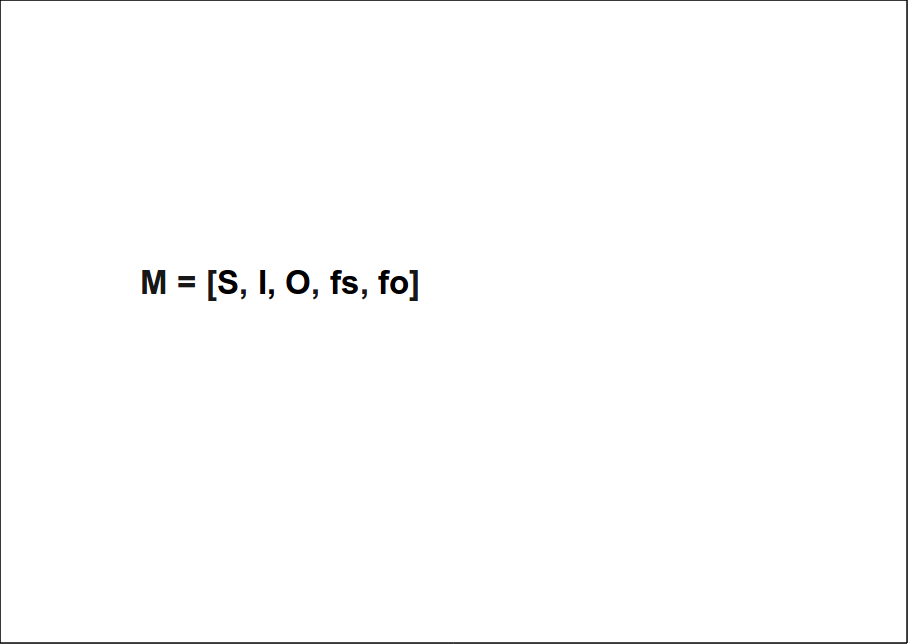
\includegraphics[height=2.7in, width=4in]{images/entendendo_definicao_1.png}
\end{frame}

\begin{frame}
  \frametitle{Definição}
    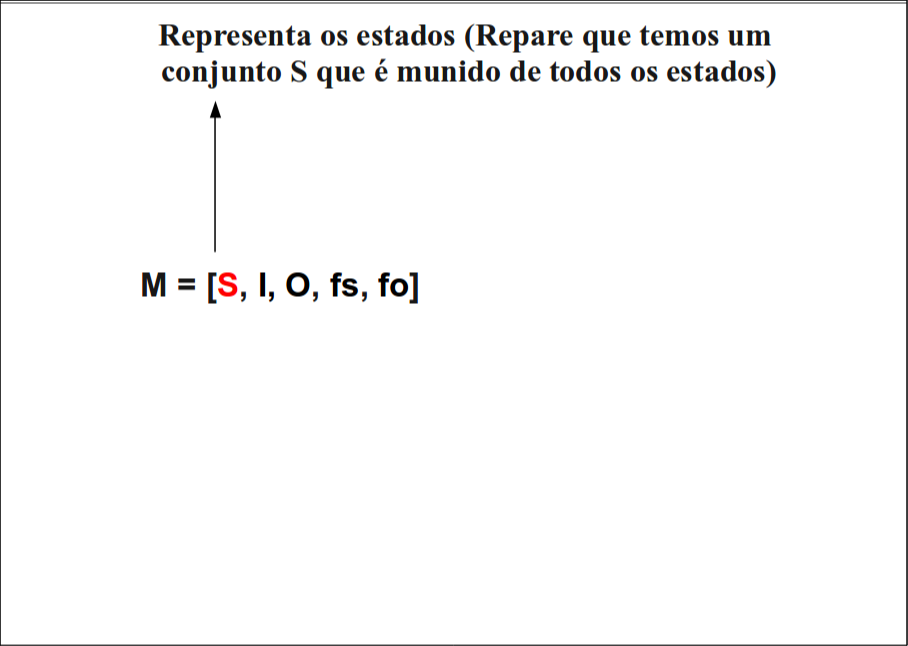
\includegraphics[height=2.7in, width=4in]{images/entendendo_definicao_2.png}
\end{frame}

\begin{frame}
  \frametitle{Definição}
    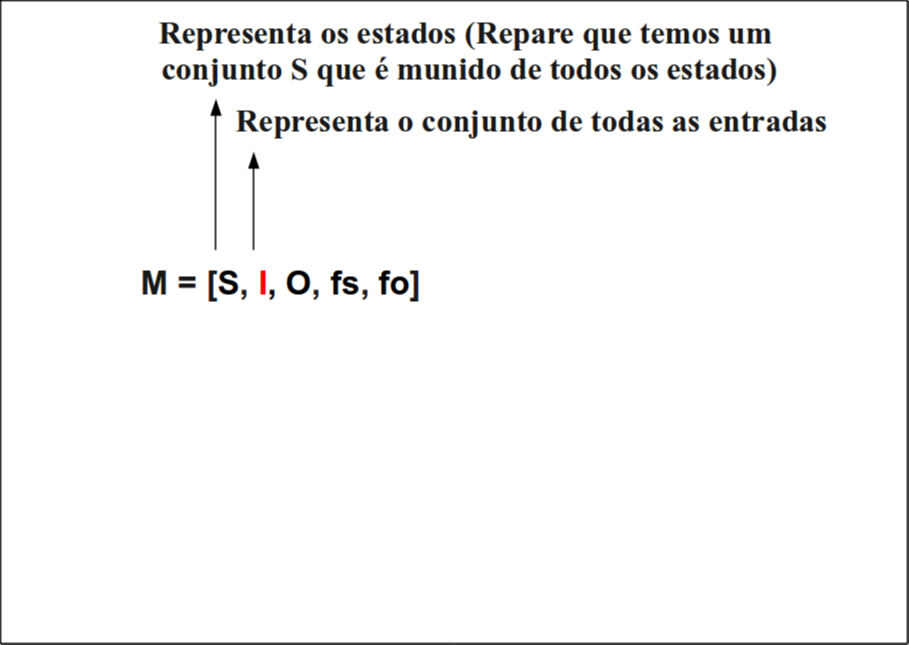
\includegraphics[height=2.7in, width=4in]{images/entendendo_definicao_3.png}
\end{frame}

\begin{frame}
  \frametitle{Definição}
    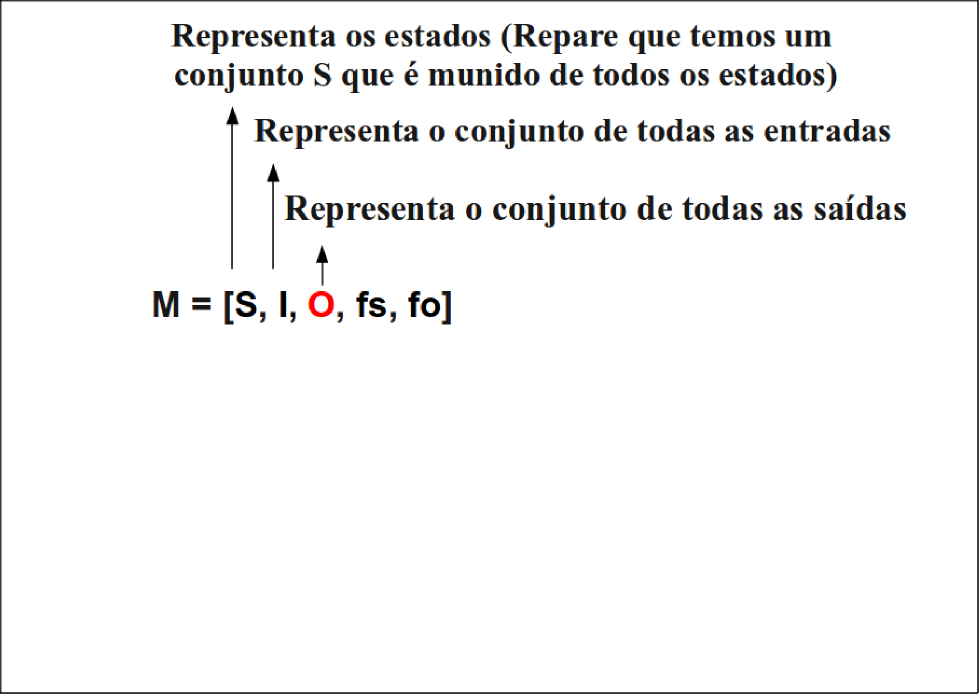
\includegraphics[height=2.7in, width=4in]{images/entendendo_definicao_4.png}
\end{frame}

\begin{frame}
  \frametitle{Definição}
    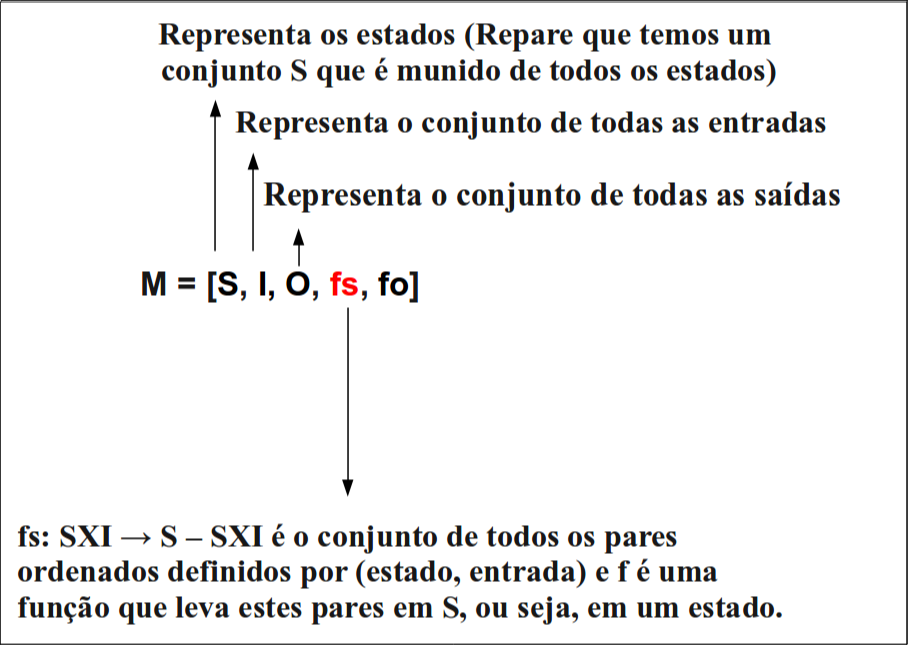
\includegraphics[height=2.7in, width=4in]{images/entendendo_definicao_5.png}
\end{frame}

\begin{frame}
  \frametitle{Definição}
    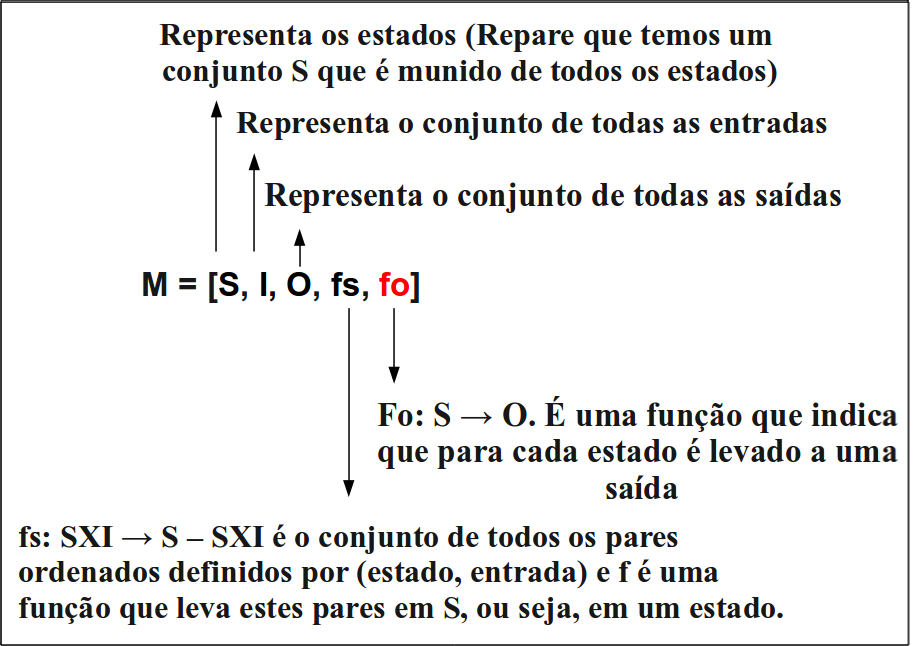
\includegraphics[height=2.7in, width=4in]{images/entendendo_definicao_6.png}
\end{frame}

%SEÇÃO == BIBLIOGRAFIA
\section{Bibliografia}
\begin{frame}
  \frametitle{Referências bibliográficas}
  \begin{enumerate}
    \item Fundamentos Matemáticos para a Ciência da computação - Judith L 
      Gersting
    \end{enumerate}
\end{frame}

\end{document}
